\documentclass[border=12pt]{standalone}
\usepackage[utf8]{inputenc}
\usepackage[utf8]{vietnam}
\usepackage{amsmath,amsfonts,amssymb}
\usepackage{siunitx}
\usepackage{tikz}
\usetikzlibrary{arrows, decorations.markings, calc, fadings, decorations.pathreplacing, patterns, decorations.pathmorphing, positioning}
\begin{document}
	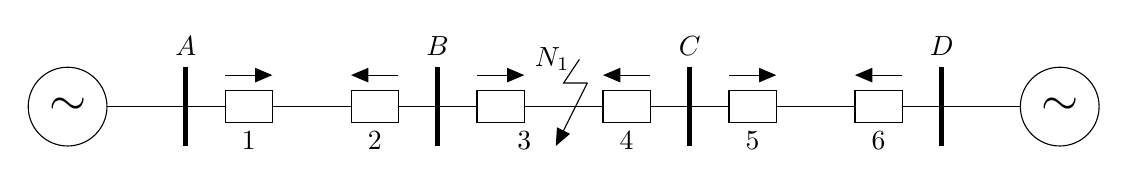
\begin{tikzpicture}[>=triangle 45]
		\draw (0,0) circle (.5)  node{\LARGE{$\mathbf{\sim}$}};
		\draw (0.5, 0) -- (1.5,0);
		\draw[ultra thick] (1.5,0.5) node[above]{$A$} -- (1.5, -.5);
		\draw (1.5, 0) -- (2, 0); \draw (2,0.2) rectangle (2.6,-0.2); \draw (2.3,-.2) node[below]{$1$}; \draw (2.6, 0) -- (3.6,0);\draw (3.6,0.2) rectangle (4.2,-0.2); \draw (3.9,-.2) node[below]{$2$}; \draw (4.2,0) -- (4.7,0); \draw[->] (2,0.4) -- (2.6,0.4); \draw[<-] (3.6,0.4) -- (4.2,0.4);
					
		\draw[ultra thick] (4.7,0.5) node[above]{$B$} -- (4.7, -.5);
		\draw (4.7, 0) -- (5.2, 0); \draw (5.2,0.2) rectangle (5.8,-0.2); \draw (5.8,-.2) node[below]{$3$}; \draw (5.8, 0) -- (6.8,0);\draw (6.8,0.2) rectangle (7.4,-0.2); \draw (7.1,-.2) node[below]{$4$}; \draw (7.4,0) -- (7.9,0); \draw[->] (5.2,0.4) -- (5.8,0.4); \draw[<-] (6.8,0.4) -- (7.4,0.4); \draw (6.5,0.6) node[left]{$N_1$} -- (6.3,0.3) -- (6.6,0.3); \draw[->] (6.6,0.3) -- (6.2,-.5);
					
		\draw[ultra thick] (7.9,0.5) node[above]{$C$} -- (7.9, -.5); 
		\draw (7.9, 0) -- (8.4, 0); \draw (8.4,0.2) rectangle (9,-0.2); \draw (8.7,-.2) node[below]{$5$}; \draw (9, 0) -- (10,0);\draw (10,0.2) rectangle (10.6,-0.2); \draw (10.3,-.2) node[below]{$6$}; \draw (10.6,0) -- (11.1,0); \draw[->] (8.4,0.4) -- (9,0.4); \draw[<-] (10,0.4) -- (10.6,0.4);
					
		\draw[ultra thick] (11.1,0.5) node[above]{$D$} -- (11.1, -.5);
					
		\draw (11.1, 0) -- (12.1, 0); \draw (12.6,0) circle (.5)  node{\LARGE{$\mathbf{\sim}$}};
	\end{tikzpicture}
\end{document} 